% Options for packages loaded elsewhere
\PassOptionsToPackage{unicode}{hyperref}
\PassOptionsToPackage{hyphens}{url}
\PassOptionsToPackage{dvipsnames,svgnames,x11names}{xcolor}
%
\documentclass[
  letterpaper,
  DIV=11,
  numbers=noendperiod]{scrartcl}

\usepackage{amsmath,amssymb}
\usepackage{lmodern}
\usepackage{iftex}
\ifPDFTeX
  \usepackage[T1]{fontenc}
  \usepackage[utf8]{inputenc}
  \usepackage{textcomp} % provide euro and other symbols
\else % if luatex or xetex
  \usepackage{unicode-math}
  \defaultfontfeatures{Scale=MatchLowercase}
  \defaultfontfeatures[\rmfamily]{Ligatures=TeX,Scale=1}
\fi
% Use upquote if available, for straight quotes in verbatim environments
\IfFileExists{upquote.sty}{\usepackage{upquote}}{}
\IfFileExists{microtype.sty}{% use microtype if available
  \usepackage[]{microtype}
  \UseMicrotypeSet[protrusion]{basicmath} % disable protrusion for tt fonts
}{}
\makeatletter
\@ifundefined{KOMAClassName}{% if non-KOMA class
  \IfFileExists{parskip.sty}{%
    \usepackage{parskip}
  }{% else
    \setlength{\parindent}{0pt}
    \setlength{\parskip}{6pt plus 2pt minus 1pt}}
}{% if KOMA class
  \KOMAoptions{parskip=half}}
\makeatother
\usepackage{xcolor}
\setlength{\emergencystretch}{3em} % prevent overfull lines
\setcounter{secnumdepth}{-\maxdimen} % remove section numbering
% Make \paragraph and \subparagraph free-standing
\ifx\paragraph\undefined\else
  \let\oldparagraph\paragraph
  \renewcommand{\paragraph}[1]{\oldparagraph{#1}\mbox{}}
\fi
\ifx\subparagraph\undefined\else
  \let\oldsubparagraph\subparagraph
  \renewcommand{\subparagraph}[1]{\oldsubparagraph{#1}\mbox{}}
\fi

\usepackage{color}
\usepackage{fancyvrb}
\newcommand{\VerbBar}{|}
\newcommand{\VERB}{\Verb[commandchars=\\\{\}]}
\DefineVerbatimEnvironment{Highlighting}{Verbatim}{commandchars=\\\{\}}
% Add ',fontsize=\small' for more characters per line
\usepackage{framed}
\definecolor{shadecolor}{RGB}{241,243,245}
\newenvironment{Shaded}{\begin{snugshade}}{\end{snugshade}}
\newcommand{\AlertTok}[1]{\textcolor[rgb]{0.68,0.00,0.00}{#1}}
\newcommand{\AnnotationTok}[1]{\textcolor[rgb]{0.37,0.37,0.37}{#1}}
\newcommand{\AttributeTok}[1]{\textcolor[rgb]{0.40,0.45,0.13}{#1}}
\newcommand{\BaseNTok}[1]{\textcolor[rgb]{0.68,0.00,0.00}{#1}}
\newcommand{\BuiltInTok}[1]{\textcolor[rgb]{0.00,0.23,0.31}{#1}}
\newcommand{\CharTok}[1]{\textcolor[rgb]{0.13,0.47,0.30}{#1}}
\newcommand{\CommentTok}[1]{\textcolor[rgb]{0.37,0.37,0.37}{#1}}
\newcommand{\CommentVarTok}[1]{\textcolor[rgb]{0.37,0.37,0.37}{\textit{#1}}}
\newcommand{\ConstantTok}[1]{\textcolor[rgb]{0.56,0.35,0.01}{#1}}
\newcommand{\ControlFlowTok}[1]{\textcolor[rgb]{0.00,0.23,0.31}{#1}}
\newcommand{\DataTypeTok}[1]{\textcolor[rgb]{0.68,0.00,0.00}{#1}}
\newcommand{\DecValTok}[1]{\textcolor[rgb]{0.68,0.00,0.00}{#1}}
\newcommand{\DocumentationTok}[1]{\textcolor[rgb]{0.37,0.37,0.37}{\textit{#1}}}
\newcommand{\ErrorTok}[1]{\textcolor[rgb]{0.68,0.00,0.00}{#1}}
\newcommand{\ExtensionTok}[1]{\textcolor[rgb]{0.00,0.23,0.31}{#1}}
\newcommand{\FloatTok}[1]{\textcolor[rgb]{0.68,0.00,0.00}{#1}}
\newcommand{\FunctionTok}[1]{\textcolor[rgb]{0.28,0.35,0.67}{#1}}
\newcommand{\ImportTok}[1]{\textcolor[rgb]{0.00,0.46,0.62}{#1}}
\newcommand{\InformationTok}[1]{\textcolor[rgb]{0.37,0.37,0.37}{#1}}
\newcommand{\KeywordTok}[1]{\textcolor[rgb]{0.00,0.23,0.31}{#1}}
\newcommand{\NormalTok}[1]{\textcolor[rgb]{0.00,0.23,0.31}{#1}}
\newcommand{\OperatorTok}[1]{\textcolor[rgb]{0.37,0.37,0.37}{#1}}
\newcommand{\OtherTok}[1]{\textcolor[rgb]{0.00,0.23,0.31}{#1}}
\newcommand{\PreprocessorTok}[1]{\textcolor[rgb]{0.68,0.00,0.00}{#1}}
\newcommand{\RegionMarkerTok}[1]{\textcolor[rgb]{0.00,0.23,0.31}{#1}}
\newcommand{\SpecialCharTok}[1]{\textcolor[rgb]{0.37,0.37,0.37}{#1}}
\newcommand{\SpecialStringTok}[1]{\textcolor[rgb]{0.13,0.47,0.30}{#1}}
\newcommand{\StringTok}[1]{\textcolor[rgb]{0.13,0.47,0.30}{#1}}
\newcommand{\VariableTok}[1]{\textcolor[rgb]{0.07,0.07,0.07}{#1}}
\newcommand{\VerbatimStringTok}[1]{\textcolor[rgb]{0.13,0.47,0.30}{#1}}
\newcommand{\WarningTok}[1]{\textcolor[rgb]{0.37,0.37,0.37}{\textit{#1}}}

\providecommand{\tightlist}{%
  \setlength{\itemsep}{0pt}\setlength{\parskip}{0pt}}\usepackage{longtable,booktabs,array}
\usepackage{calc} % for calculating minipage widths
% Correct order of tables after \paragraph or \subparagraph
\usepackage{etoolbox}
\makeatletter
\patchcmd\longtable{\par}{\if@noskipsec\mbox{}\fi\par}{}{}
\makeatother
% Allow footnotes in longtable head/foot
\IfFileExists{footnotehyper.sty}{\usepackage{footnotehyper}}{\usepackage{footnote}}
\makesavenoteenv{longtable}
\usepackage{graphicx}
\makeatletter
\def\maxwidth{\ifdim\Gin@nat@width>\linewidth\linewidth\else\Gin@nat@width\fi}
\def\maxheight{\ifdim\Gin@nat@height>\textheight\textheight\else\Gin@nat@height\fi}
\makeatother
% Scale images if necessary, so that they will not overflow the page
% margins by default, and it is still possible to overwrite the defaults
% using explicit options in \includegraphics[width, height, ...]{}
\setkeys{Gin}{width=\maxwidth,height=\maxheight,keepaspectratio}
% Set default figure placement to htbp
\makeatletter
\def\fps@figure{htbp}
\makeatother

\usepackage{fvextra}
\usepackage{svg}
\DefineVerbatimEnvironment{Highlighting}{Verbatim}{breaklines,commandchars=\\\{\}}
\KOMAoption{captions}{tableheading}
\makeatletter
\makeatother
\makeatletter
\makeatother
\makeatletter
\@ifpackageloaded{caption}{}{\usepackage{caption}}
\AtBeginDocument{%
\ifdefined\contentsname
  \renewcommand*\contentsname{Table of contents}
\else
  \newcommand\contentsname{Table of contents}
\fi
\ifdefined\listfigurename
  \renewcommand*\listfigurename{List of Figures}
\else
  \newcommand\listfigurename{List of Figures}
\fi
\ifdefined\listtablename
  \renewcommand*\listtablename{List of Tables}
\else
  \newcommand\listtablename{List of Tables}
\fi
\ifdefined\figurename
  \renewcommand*\figurename{Figure}
\else
  \newcommand\figurename{Figure}
\fi
\ifdefined\tablename
  \renewcommand*\tablename{Table}
\else
  \newcommand\tablename{Table}
\fi
}
\@ifpackageloaded{float}{}{\usepackage{float}}
\floatstyle{ruled}
\@ifundefined{c@chapter}{\newfloat{codelisting}{h}{lop}}{\newfloat{codelisting}{h}{lop}[chapter]}
\floatname{codelisting}{Listing}
\newcommand*\listoflistings{\listof{codelisting}{List of Listings}}
\makeatother
\makeatletter
\@ifpackageloaded{caption}{}{\usepackage{caption}}
\@ifpackageloaded{subcaption}{}{\usepackage{subcaption}}
\makeatother
\makeatletter
\@ifpackageloaded{tcolorbox}{}{\usepackage[many]{tcolorbox}}
\makeatother
\makeatletter
\@ifundefined{shadecolor}{\definecolor{shadecolor}{rgb}{.97, .97, .97}}
\makeatother
\makeatletter
\makeatother
\ifLuaTeX
  \usepackage{selnolig}  % disable illegal ligatures
\fi
\IfFileExists{bookmark.sty}{\usepackage{bookmark}}{\usepackage{hyperref}}
\IfFileExists{xurl.sty}{\usepackage{xurl}}{} % add URL line breaks if available
\urlstyle{same} % disable monospaced font for URLs
\hypersetup{
  colorlinks=true,
  linkcolor={blue},
  filecolor={Maroon},
  citecolor={Blue},
  urlcolor={Blue},
  pdfcreator={LaTeX via pandoc}}

\author{}
\date{}

\begin{document}
\begin{titlepage}

    \newcommand{\HRule}{\rule{\linewidth}{0.5mm}}
    
    \center
    
    \textsc{\LARGE GSMST }\\[0.3cm]
    \textsc{\Large Applications of Linear Algebra }\\[0.3cm]
    \textsc{\Large in Programming}\\[0.5cm]
    
    \HRule \\[0.4cm]
    { \huge \bfseries Error Correcting Lab}\\[0.03cm]
    \HRule \\[1.5cm]
    
    \begin{minipage}{0.4\textwidth}
    \begin{flushleft} \large
    \emph{Submitted By:}\\
    Anish Goyal \\4th Period
    \end{flushleft}
    \end{minipage}
    ~
    \begin{minipage}{0.4\textwidth}
    \begin{flushright} \large
    \emph{Submitted To:} \\
    Mrs. Denise Stiffler\\Educator
    \end{flushright}
    \end{minipage}\\[1cm]
    
    {\large May 8, 2023}\\[1cm]
    
    
\includegraphics{logo.png}\\[1cm]
    \vfill
    \end{titlepage}
\newpage

\ifdefined\Shaded\renewenvironment{Shaded}{\begin{tcolorbox}[borderline west={3pt}{0pt}{shadecolor}, interior hidden, boxrule=0pt, enhanced, breakable, frame hidden, sharp corners]}{\end{tcolorbox}}\fi

\renewcommand*\contentsname{Table of contents}
{
\hypersetup{linkcolor=}
\setcounter{tocdepth}{4}
\tableofcontents
}
\newpage{}

\hypertarget{review-questions}{%
\section{\texorpdfstring{\textbf{2.13 Review
Questions}}{2.13 Review Questions}}\label{review-questions}}

\hypertarget{what-is-vector-addition}{%
\subsection{What is vector addition?}\label{what-is-vector-addition}}

Vector addition is the adding of two vectors of the same size into a
single vector. Say we have two vectors \(v\) and \(k\). The addition of
the vectors \(v\) and \(k\) can be defined as follows:\\
\([u_1, u_2, ..., u_n]+[v_1, v_2, ..., v_n] = [u_1+v_1, u_2+v_2, ..., u_n+v_n]\)

\hypertarget{what-is-the-geometric-interpretation-of-vector-addition}{%
\subsection{What is the geometric interpretation of vector
addition?}\label{what-is-the-geometric-interpretation-of-vector-addition}}

The geometric interpretation of vector addition is placing the tail of
the second vector at the head of the first vector and drawing a new
vector from the tail of the first vector to the head of the second
vector, which represents the sum of the two vectors.

\hypertarget{what-is-scalar-vector-multiplication}{%
\subsection{What is scalar-vector
multiplication?}\label{what-is-scalar-vector-multiplication}}

Scalar-vector multiplication is an operation performed between a scalar
value and a vector that results in a new vector. The scalar multiplies
each component of the vector, which results in a new vector that has the
same direction as the original director, but with a length (or
magnitude) that is scaled by that scalar value.

\hypertarget{what-is-the-distributive-property-that-involves-scalar-vector-multiplication-but-not-vector-addition}{%
\subsection{What is the distributive property that involves
scalar-vector multiplication but not vector
addition?}\label{what-is-the-distributive-property-that-involves-scalar-vector-multiplication-but-not-vector-addition}}

The distributive property that involves scalar-vector multiplication but
not vector addition is:\\
\((\alpha + \beta)u = \alpha u + \beta u\)\\
where \(\alpha\) and \(\beta\) are scalars and \(u\) is a vector. This
property states that when a vector is multiplied by the sum of two
scalars, the result is equivalent to the sum of the scalar
multiplication of one scalar to that vector and the scalar
multiplication of the other scalar to that vector.

\hypertarget{what-is-the-distributive-property-that-involves-both-scalar-vector-multiplication-and-vector-addition}{%
\subsection{What is the distributive property that involves both
scalar-vector multiplication and vector
addition?}\label{what-is-the-distributive-property-that-involves-both-scalar-vector-multiplication-and-vector-addition}}

The distributive property that involves both scalar-vector
multiplication and vector addition is:\\
\(a \cdot (u + v) = a \cdot u + a \cdot v\)\\
where \(a\) is a scalar, and \(u\) and \(v\) are vectors. This property
states that when a scalar is multiplied to the sum of two vectors, the
result is equivalent to the sum of the scalar multiplication to each of
those vectors. In other words, you can distribute a scalar over the sum
of two vectors, and the resulting vector will be the same as adding the
scalar multiples to each vector separately.

\hypertarget{how-is-scalar-vector-multiplication-used-to-represent-the-line-through-a-pair-of-given-points}{%
\subsection{How is scalar-vector multiplication used to represent the
line through a pair of given
points?}\label{how-is-scalar-vector-multiplication-used-to-represent-the-line-through-a-pair-of-given-points}}

The line through a pair of given points \(u\) and \(v\), known as the
\(u\)-to-\(v\) line segment, consists of the set of convex combinations
of \(u\) where
\(\{\alpha v + \beta u : \alpha, \beta \in \mathbb{R}, \alpha, \beta \geq 0, \alpha + \beta = 1\}\).

\hypertarget{what-is-dot-product}{%
\subsection{What is dot product?}\label{what-is-dot-product}}

The dot product is defined as the sum of the elements with the same
index multiplied together across two vectors with equal length.

\hypertarget{what-is-the-homogeneity-property-that-relates-dot-product-to-scalar-vector-multiplication}{%
\subsection{\texorpdfstring{What is the \emph{homogeneity} property that
relates dot-product to scalar-vector
multiplication?}{What is the homogeneity property that relates dot-product to scalar-vector multiplication?}}\label{what-is-the-homogeneity-property-that-relates-dot-product-to-scalar-vector-multiplication}}

The \emph{homogeneity} property says multiplying one of the vectors
being dot-producted together by a scalar is equivalent to multiplying
that scalar to the actual dot product:\\
\((\alpha u) \cdot v = \alpha (u \cdot v)\)

\hypertarget{what-is-the-distributive-property-property-that-relates-dot-product-to-vector-addition}{%
\subsection{What is the distributive property property that relates
dot-product to vector
addition?}\label{what-is-the-distributive-property-property-that-relates-dot-product-to-vector-addition}}

Dot product is distributive over vector addition:\\
\((u + v) \cdot w = u \cdot w + v \cdot w\)

\hypertarget{what-is-a-linear-equation-expressed-using-dot-product}{%
\subsection{What is a linear equation (expressed using
dot-product)?}\label{what-is-a-linear-equation-expressed-using-dot-product}}

A linear equation expressed using dot product involves finding a scalar
product of a vector x and a vector w, and comparing it to a scalar value
b. This can be written as:\\
\(a \cdot x = \beta\)\\
where \(a\) is a vector, \(x\) is a vector variable, and \(\beta\) is a
scalar.

\hypertarget{what-is-a-linear-system}{%
\subsection{What is a linear system?}\label{what-is-a-linear-system}}

A linear system is a list of linear equations with the same vector
variable expressed using dot-product:\\
\(a_1 \cdot x = \beta_1\)\\
\(a_2 \cdot x = \beta_2\)\\
\(...\)\\
\(a_m \cdot x = \beta_m\)

\hypertarget{what-is-an-upper-triangular-linear-system}{%
\subsection{What is an upper-triangular linear
system?}\label{what-is-an-upper-triangular-linear-system}}

An upper-triangular linear system is a linear system that is in
row-echelon form with zeros across the scalar values of the bottom left
triangle.

\hypertarget{how-can-one-solve-an-upper-triangular-linear-system}{%
\subsection{How can one solve an upper-triangular linear
system?}\label{how-can-one-solve-an-upper-triangular-linear-system}}

You can solve an upper-triangle linear system with Gaussian Elimination
with backwards substitution. Once you have solved for a single scalar at
the bottommost equation of the linear system, you can plug in that
scalar into the following equations and work your way up.

\hypertarget{problems}{%
\section{\texorpdfstring{\textbf{2.14
Problems}}{2.14 Problems}}\label{problems}}

\hypertarget{vector-addition-practice}{%
\subsection{Vector addition practice}\label{vector-addition-practice}}

\hypertarget{problem-2.14.1}{%
\subsubsection{Problem 2.14.1}\label{problem-2.14.1}}

For vectors \(v = [-1, 3]\) and \(u = [0, 4]\), find the vectors
\(v+u\), \(v-u\), and \(3v-2u\). Draw these arrows as arrows on the same
graph.

\(v+u\) = {[}-1, 7{]}\\
\(v-u\) = {[}-1, -1{]}\\
\(3v-2u\) = {[}-3, 1{]}

\begin{Shaded}
\begin{Highlighting}[numbers=left,,]
\ImportTok{import}\NormalTok{ matplotlib.pyplot }\ImportTok{as}\NormalTok{ plt}

\NormalTok{v }\OperatorTok{=}\NormalTok{ [}\OperatorTok{{-}}\DecValTok{1}\NormalTok{, }\DecValTok{3}\NormalTok{]}
\NormalTok{u }\OperatorTok{=}\NormalTok{ [}\DecValTok{0}\NormalTok{, }\DecValTok{4}\NormalTok{]}
\NormalTok{v\_plus\_u }\OperatorTok{=}\NormalTok{ [}\OperatorTok{{-}}\DecValTok{1}\NormalTok{, }\DecValTok{7}\NormalTok{]}
\NormalTok{v\_minus\_u }\OperatorTok{=}\NormalTok{ [}\OperatorTok{{-}}\DecValTok{1}\NormalTok{, }\OperatorTok{{-}}\DecValTok{1}\NormalTok{]}
\NormalTok{three\_v\_minus\_two\_u }\OperatorTok{=}\NormalTok{ [}\OperatorTok{{-}}\DecValTok{3}\NormalTok{, }\OperatorTok{{-}}\DecValTok{5}\NormalTok{]}

\NormalTok{plt.arrow(}\DecValTok{0}\NormalTok{, }\DecValTok{0}\NormalTok{, v[}\DecValTok{0}\NormalTok{], v[}\DecValTok{1}\NormalTok{], color}\OperatorTok{=}\StringTok{\textquotesingle{}blue\textquotesingle{}}\NormalTok{, width}\OperatorTok{=}\FloatTok{0.05}\NormalTok{, length\_includes\_head}\OperatorTok{=}\VariableTok{True}\NormalTok{, label}\OperatorTok{=}\StringTok{\textquotesingle{}v\textquotesingle{}}\NormalTok{)}
\NormalTok{plt.arrow(}\DecValTok{0}\NormalTok{, }\DecValTok{0}\NormalTok{, u[}\DecValTok{0}\NormalTok{], u[}\DecValTok{1}\NormalTok{], color}\OperatorTok{=}\StringTok{\textquotesingle{}green\textquotesingle{}}\NormalTok{, width}\OperatorTok{=}\FloatTok{0.05}\NormalTok{, length\_includes\_head}\OperatorTok{=}\VariableTok{True}\NormalTok{, label}\OperatorTok{=}\StringTok{\textquotesingle{}u\textquotesingle{}}\NormalTok{)}
\NormalTok{plt.arrow(}\DecValTok{0}\NormalTok{, }\DecValTok{0}\NormalTok{, v\_plus\_u[}\DecValTok{0}\NormalTok{], v\_plus\_u[}\DecValTok{1}\NormalTok{], color}\OperatorTok{=}\StringTok{\textquotesingle{}red\textquotesingle{}}\NormalTok{, width}\OperatorTok{=}\FloatTok{0.05}\NormalTok{, length\_includes\_head}\OperatorTok{=}\VariableTok{True}\NormalTok{, label}\OperatorTok{=}\StringTok{\textquotesingle{}v+u\textquotesingle{}}\NormalTok{)}
\NormalTok{plt.arrow(}\DecValTok{0}\NormalTok{, }\DecValTok{0}\NormalTok{, v\_minus\_u[}\DecValTok{0}\NormalTok{], v\_minus\_u[}\DecValTok{1}\NormalTok{], color}\OperatorTok{=}\StringTok{\textquotesingle{}purple\textquotesingle{}}\NormalTok{, width}\OperatorTok{=}\FloatTok{0.05}\NormalTok{, length\_includes\_head}\OperatorTok{=}\VariableTok{True}\NormalTok{, label}\OperatorTok{=}\StringTok{\textquotesingle{}v{-}u\textquotesingle{}}\NormalTok{)}
\NormalTok{plt.arrow(}\DecValTok{0}\NormalTok{, }\DecValTok{0}\NormalTok{, three\_v\_minus\_two\_u[}\DecValTok{0}\NormalTok{], three\_v\_minus\_two\_u[}\DecValTok{1}\NormalTok{], color}\OperatorTok{=}\StringTok{\textquotesingle{}orange\textquotesingle{}}\NormalTok{, width}\OperatorTok{=}\FloatTok{0.05}\NormalTok{, length\_includes\_head}\OperatorTok{=}\VariableTok{True}\NormalTok{, label}\OperatorTok{=}\StringTok{\textquotesingle{}3v{-}2u\textquotesingle{}}\NormalTok{)}

\NormalTok{plt.xlim(}\OperatorTok{{-}}\DecValTok{4}\NormalTok{, }\DecValTok{2}\NormalTok{)}
\NormalTok{plt.ylim(}\OperatorTok{{-}}\DecValTok{6}\NormalTok{, }\DecValTok{8}\NormalTok{)}

\NormalTok{plt.legend()}
\NormalTok{plt.show()}
\end{Highlighting}
\end{Shaded}

\begin{figure}[H]

{\centering 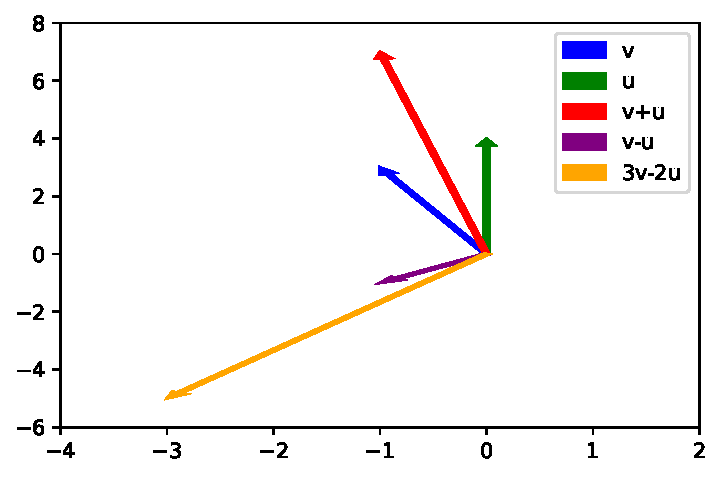
\includegraphics{Chapter-2-Assignment_files/figure-pdf/cell-2-output-1.pdf}

}

\end{figure}

\hypertarget{problem-2.14.2}{%
\subsubsection{Problem 2.14.2}\label{problem-2.14.2}}

Given the vectors \(v = [2, -1, 5]\) and \(u = [-1, 1, 1]\), find the
vectors \(v+u\), \(v-u\), \(2v-u\), and \(v+2u\).

\(v+u = [1, 0, 6]\)\\
\(v-u = [3, -2, 4]\) ~ \(2v-u = [5, -3, 9]\)\\
\(v+2u = [0, 1, 7]\)

\hypertarget{problem-2.14.3}{%
\subsubsection{Problem 2.14.3}\label{problem-2.14.3}}

For the vectors \(v=[0, one, one]\) and \(u=[one, one, one]\) over
\(GF(2)\), find \(v+u\) and \(v+u+u\).

\(v+u = [0, one, one] + [one, one, one] = [one, 0, 0]\)\\
\(v+u+u = [one, 0, 0] + [one, one, one] = [0, one, one]\)

\hypertarget{expressing-one-gf2-vector-as-a-sum-of-others}{%
\subsection{\texorpdfstring{Expressing one \(GF(2)\) vector as a sum of
others}{Expressing one GF(2) vector as a sum of others}}\label{expressing-one-gf2-vector-as-a-sum-of-others}}

\hypertarget{problem-2.14.4}{%
\subsubsection{Problem 2.14.4}\label{problem-2.14.4}}

Here are six 7-vectors over \(GF(2)\):

\begin{longtable}[]{@{}ll@{}}
\toprule()
\endhead
\textbf{a} = 1100000 & \textbf{d} = 0001100 \\
\textbf{b} = 0110000 & \textbf{e} = 0000110 \\
\textbf{c} = 0011000 & \textbf{f} = 0000011 \\
\bottomrule()
\end{longtable}

For each of the following vectors \(u\), find a subset of the above
vectors whose sum is \(u\), or report that no such subset exists.

\begin{enumerate}
\def\labelenumi{\arabic{enumi}.}
\tightlist
\item
  \(u\) = 0010010\\
\item
  \(u\) = 0100010\\
\end{enumerate}

\begin{enumerate}
\def\labelenumi{\arabic{enumi})}
\tightlist
\item
  \(u\) = \(c\) + \(d\) + \(e\)\\
\item
  \(u\) = \(b\) + \(c\) + \(d\) + \(e\)
\end{enumerate}

\hypertarget{problem-2.14.5}{%
\subsubsection{Problem 2.14.5}\label{problem-2.14.5}}

Here are six 7-vectors over \(GF(2)\):

\begin{longtable}[]{@{}ll@{}}
\toprule()
\endhead
\textbf{a} = 1110000 & \textbf{d} = 0001110 \\
\textbf{b} = 0111000 & \textbf{e} = 0000111 \\
\textbf{c} = 0011100 & \textbf{f} = 0000011 \\
\bottomrule()
\end{longtable}

For each of the following vectors \(u\), find a subset of the above
vectors whose sum is \(u\), or report that no such subset exists.

\begin{enumerate}
\def\labelenumi{\arabic{enumi}.}
\tightlist
\item
  \(u\) = 0010010\\
\item
  \(u\) = 0100010 ~
\end{enumerate}

\begin{enumerate}
\def\labelenumi{\arabic{enumi})}
\tightlist
\item
  \(u\) = \(c\) + \(d\)\\
\item
  There is no such subset.
\end{enumerate}

\hypertarget{finding-a-solution-to-linear-equations-over-gf2}{%
\subsection{\texorpdfstring{Finding a solution to linear equations over
\(GF(2)\)}{Finding a solution to linear equations over GF(2)}}\label{finding-a-solution-to-linear-equations-over-gf2}}

\hypertarget{problem-2.14.6}{%
\subsubsection{Problem 2.14.6}\label{problem-2.14.6}}

Find a vector \(x = [x_1, x_2, x_3, x_4]\) over \(GF(2)\) satisfying the
following linear equations:\\
\(1100 \cdot x = 1\)\\
\(1010 \cdot x = 1\) ~ \(1111 \cdot x = 1\)\\
Show that \(x + 1111\) also satisfies the equations.\\

A vector that satisfies the linear equation is \(x = [1, 0, 0, 0]\).
\(1100 \cdot 1000 \stackrel{\checkmark}{=} 1\)\\
\(1010 \cdot 1000 \stackrel{\checkmark}{=} 1\)\\
\(1111 \cdot 1000 \stackrel{\checkmark}{=} 1\)\\
\((x=1000)+1111 = 0111\) also satisfies the equations:\\
\(1100 \cdot 0111 \stackrel{\checkmark}{=} 0 + 1 + 0 + 0 \stackrel{\checkmark}{=} 1\)\\
\(1010 \cdot 0111 \stackrel{\checkmark}{=} 0 + 0 + 1 + 0 \stackrel{\checkmark}{=} 1\)\\
\(1111 \cdot 0111 \stackrel{\checkmark}{=} 0 + 1 + 1 + 1 \stackrel{\checkmark}{=} 1\)

\hypertarget{formulating-equations-using-dot-product}{%
\subsection{Formulating equations using
dot-product}\label{formulating-equations-using-dot-product}}

\hypertarget{problem-2.14.7}{%
\subsubsection{Problem 2.14.7}\label{problem-2.14.7}}

Consider the equations\\
\(2x_0 + 3x_1 - 4x_2 + x_3 = 10\)\\
\(x_0 - 5x_1 + 2x_2 + 0x_3 = 35\)\\
\(4x_0 + x_1 - x_2 - x_3 = 8\)\\
Your job is not to solve these equations but to formulate them using
dot-product. In particular, come up with three vectors v1, v2, and v3
represented as lists so that the above equations are equivalent to\\
\(\mathrm{v1} \cdot x = 10\)\\
\(\mathrm{v2} \cdot x = 35\)\\
\(\mathrm{v3} \cdot x = 8\)\\
where \(x\) is a 4-vector over \(\mathbb{R}\).\\
\(v_1=[2, 3, -4, 1]\)\\
\(v_2=[1, -5, 2, 0]\)\\
\(v_3=[4, 1, -1, -1]\)

\hypertarget{plotting-lines-and-segments}{%
\subsection{Plotting lines and
segments}\label{plotting-lines-and-segments}}

\hypertarget{problem-2.14.8}{%
\subsubsection{Problem 2.14.8}\label{problem-2.14.8}}

Use the \texttt{plot} module to plot\\
(a) a substantial portion of the line through {[}-1.5, 2{]} and {[}3,
0{]}, and\\
(b) the line segment between {[}2, 1{]} and {[}-2, 2{]}.\\
For each, provide the Python statements you used and the plot obtained.

\begin{Shaded}
\begin{Highlighting}[numbers=left,,]
\ImportTok{from}\NormalTok{ plotting }\ImportTok{import} \OperatorTok{*}
\ImportTok{from}\NormalTok{ IPython.display }\ImportTok{import}\NormalTok{ SVG, display}
\NormalTok{L}\OperatorTok{=}\NormalTok{[(}\DecValTok{3} \OperatorTok{+}\NormalTok{ i}\OperatorTok{*}\NormalTok{(}\OperatorTok{{-}}\DecValTok{4}\NormalTok{), i}\OperatorTok{*}\DecValTok{9}\NormalTok{) }\ControlFlowTok{for}\NormalTok{ i }\KeywordTok{in} \BuiltInTok{range}\NormalTok{(}\OperatorTok{{-}}\DecValTok{20}\NormalTok{, }\DecValTok{20}\NormalTok{)]}
\NormalTok{display(SVG(plot(L, }\DecValTok{200}\NormalTok{)))}
\end{Highlighting}
\end{Shaded}

\begin{figure}[H]

{\centering \includesvg{Chapter-2-Assignment_files/figure-pdf/cell-3-output-1.svg}

}

\end{figure}

\begin{Shaded}
\begin{Highlighting}[numbers=left,,]
\ImportTok{import}\NormalTok{ numpy }\ImportTok{as}\NormalTok{ np}
\ImportTok{from}\NormalTok{ plotting }\ImportTok{import} \OperatorTok{*}
\ImportTok{from}\NormalTok{ IPython.display }\ImportTok{import}\NormalTok{ SVG, display}
\NormalTok{L}\OperatorTok{=}\NormalTok{[(}\DecValTok{2}\OperatorTok{{-}}\NormalTok{i, }\DecValTok{1}\OperatorTok{+}\FloatTok{0.25}\OperatorTok{*}\NormalTok{i) }\ControlFlowTok{for}\NormalTok{ i }\KeywordTok{in}\NormalTok{ np.arange(}\DecValTok{0}\NormalTok{, }\DecValTok{4}\NormalTok{, }\FloatTok{0.001}\NormalTok{)]}
\NormalTok{display(SVG(plot(L, }\DecValTok{3}\NormalTok{)))}
\end{Highlighting}
\end{Shaded}

\begin{figure}[H]

{\centering \includesvg{Chapter-2-Assignment_files/figure-pdf/cell-4-output-1.svg}

}

\end{figure}

\hypertarget{practice-with-dot-product}{%
\subsection{Practice with dot-product}\label{practice-with-dot-product}}

\hypertarget{problem-2.14.9}{%
\subsubsection{Problem 2.14.9}\label{problem-2.14.9}}

For each of the following pairs of vectors \(u\) and \(v\) over
\(\mathbb{R}\), evaluate the expression \(u \cdot v\):\\
(a) \(u = [1, 0], v = [5, 4321]\)\\
(b) \(u = [0, 1], v = [12345, 6]\)\\
(c) \(u = [-1, 3], v = [5, 7]\)\\
(d)
\(u = \left[-\frac{\sqrt{2}}{2}, \frac{\sqrt{2}}{2}\right], v = \left[\frac{\sqrt{2}}{2}, -\frac{\sqrt{2}}{2}\right]\)

\begin{enumerate}
\def\labelenumi{(\alph{enumi})}
\tightlist
\item
  \([1, 0] \cdot [5, 4321] = 5 + 0 = 5\)\\
\item
  \([0, 1] \cdot [12345, 6] = 0 + 6 = 6\)\\
\item
  \([-1, 3] \cdot [5, 7] = -5 + 21 =16\)\\
\item
  \(\left[-\frac{\sqrt{2}}{2}, \frac{\sqrt{2}}{2}\right] \cdot \left[\frac{\sqrt{2}}{2}, -\frac{\sqrt{2}}{2}\right] = -\frac{1}{2} - \frac{1}{2} = -1\)
\end{enumerate}

\hypertarget{writing-procedures-for-the-vec-class}{%
\subsection{\texorpdfstring{Writing procedures for the \texttt{Vec}
class}{Writing procedures for the Vec class}}\label{writing-procedures-for-the-vec-class}}

\hypertarget{problem-2.14.10}{%
\subsubsection{Problem 2.14.10}\label{problem-2.14.10}}

Download the file \texttt{vec.py} to your computer, and edit it. The
file defines procedures using the Python statement \texttt{pass}, which
does nothing. You can import the \texttt{vec} module and create
instances of \texttt{Vec} but the operations such as * and + currently
do nothing. Your job is to replace each occurrence of the \texttt{pass}
statement with appropriate code. Your code for a procedure can include
calls to others of the seven. You should make no changes to the class
definition.

\hypertarget{docstrings}{%
\paragraph{Docstrings}\label{docstrings}}

At the beginning of each procedure body is a multi-line string
(deliminated by triple quotation marks). This is called a documentation
string (\emph{docstring}). It specifies what the procedure should do.

\hypertarget{doctests}{%
\paragraph{Doctests}\label{doctests}}

The documentation string we provide for a procedure also includes
examples of the functionality that procedure is supposed to provide to
\texttt{Vec}s. The examples show an interaction with Python: statements
and expressions are evaluated by Python, and Python's responses are
shown. These examples are provided to you as tests (called
\emph{doctests}). You should make sure that your procedure is written in
such a way that the behavior of your Vec implementation matches that in
the examples. If not, your implementation is incorrect.

Download the file \texttt{vec.py} to your computer, and edit it. Fill in
the procedure definitions and test the doctests with\\
\texttt{python3\ -m\ doctest\ vec.py}.

\begin{Shaded}
\begin{Highlighting}[numbers=left,,]
\KeywordTok{def}\NormalTok{ getitem(v,k):}
    \CommentTok{"""}
\CommentTok{    Return the value of entry k in v.}
\CommentTok{    Be sure getitem(v,k) returns 0 if k is not represented in v.f.}

\CommentTok{    \textgreater{}\textgreater{}\textgreater{} v = Vec(\{\textquotesingle{}a\textquotesingle{},\textquotesingle{}b\textquotesingle{},\textquotesingle{}c\textquotesingle{}, \textquotesingle{}d\textquotesingle{}\},\{\textquotesingle{}a\textquotesingle{}:2,\textquotesingle{}c\textquotesingle{}:1,\textquotesingle{}d\textquotesingle{}:3\})}
\CommentTok{    \textgreater{}\textgreater{}\textgreater{} v[\textquotesingle{}d\textquotesingle{}]}
\CommentTok{    3}
\CommentTok{    \textgreater{}\textgreater{}\textgreater{} v[\textquotesingle{}b\textquotesingle{}]}
\CommentTok{    0}
\CommentTok{    """}
    \ControlFlowTok{assert}\NormalTok{ k }\KeywordTok{in}\NormalTok{ v.D}
    \ControlFlowTok{return}\NormalTok{ v.f[k] }\ControlFlowTok{if}\NormalTok{ k }\KeywordTok{in}\NormalTok{ v.f }\ControlFlowTok{else} \DecValTok{0}

\KeywordTok{def}\NormalTok{ setitem(v,k,val):}
    \CommentTok{"""}
\CommentTok{    Set the element of v with label d to be val.}
\CommentTok{    setitem(v,d,val) should set the value for key d even if d}
\CommentTok{    is not previously represented in v.f, and even if val is 0.}

\CommentTok{    \textgreater{}\textgreater{}\textgreater{} v = Vec(\{\textquotesingle{}a\textquotesingle{}, \textquotesingle{}b\textquotesingle{}, \textquotesingle{}c\textquotesingle{}\}, \{\textquotesingle{}b\textquotesingle{}:0\})}
\CommentTok{    \textgreater{}\textgreater{}\textgreater{} v[\textquotesingle{}b\textquotesingle{}] = 5}
\CommentTok{    \textgreater{}\textgreater{}\textgreater{} v[\textquotesingle{}b\textquotesingle{}]}
\CommentTok{    5}
\CommentTok{    \textgreater{}\textgreater{}\textgreater{} v[\textquotesingle{}a\textquotesingle{}] = 1}
\CommentTok{    \textgreater{}\textgreater{}\textgreater{} v[\textquotesingle{}a\textquotesingle{}]}
\CommentTok{    1}
\CommentTok{    \textgreater{}\textgreater{}\textgreater{} v[\textquotesingle{}a\textquotesingle{}] = 0}
\CommentTok{    \textgreater{}\textgreater{}\textgreater{} v[\textquotesingle{}a\textquotesingle{}]}
\CommentTok{    0}
\CommentTok{    """}
    \ControlFlowTok{assert}\NormalTok{ k }\KeywordTok{in}\NormalTok{ v.D}
\NormalTok{    v.f[k] }\OperatorTok{=}\NormalTok{ val}
    \ControlFlowTok{return}

\KeywordTok{def}\NormalTok{ equal(u,v):}
    \CommentTok{"""}
\CommentTok{    Return true iff u is equal to v.}
\CommentTok{    Because of sparse representation, it is not enough to compare dictionaries}

\CommentTok{    Consider using brackets notation u[...] and v[...] in your procedure}
\CommentTok{    to access entries of the input vectors.  This avoids some sparsity bugs.}

\CommentTok{    \textgreater{}\textgreater{}\textgreater{} Vec(\{\textquotesingle{}a\textquotesingle{}, \textquotesingle{}b\textquotesingle{}, \textquotesingle{}c\textquotesingle{}\}, \{\textquotesingle{}a\textquotesingle{}:0\}) == Vec(\{\textquotesingle{}a\textquotesingle{}, \textquotesingle{}b\textquotesingle{}, \textquotesingle{}c\textquotesingle{}\}, \{\textquotesingle{}b\textquotesingle{}:0\})}
\CommentTok{    True}
\CommentTok{    \textgreater{}\textgreater{}\textgreater{} Vec(\{\textquotesingle{}a\textquotesingle{}, \textquotesingle{}b\textquotesingle{}, \textquotesingle{}c\textquotesingle{}\}, \{\textquotesingle{}a\textquotesingle{}: 0\}) == Vec(\{\textquotesingle{}a\textquotesingle{}, \textquotesingle{}b\textquotesingle{}, \textquotesingle{}c\textquotesingle{}\}, \{\})}
\CommentTok{    True}
\CommentTok{    \textgreater{}\textgreater{}\textgreater{} Vec(\{\textquotesingle{}a\textquotesingle{}, \textquotesingle{}b\textquotesingle{}, \textquotesingle{}c\textquotesingle{}\}, \{\}) == Vec(\{\textquotesingle{}a\textquotesingle{}, \textquotesingle{}b\textquotesingle{}, \textquotesingle{}c\textquotesingle{}\}, \{\textquotesingle{}a\textquotesingle{}: 0\})}
\CommentTok{    True}

\CommentTok{    Be sure that equal(u, v) checks equalities for all keys from u.f and v.f even if}
\CommentTok{    some keys in u.f do not exist in v.f (or vice versa)}

\CommentTok{    \textgreater{}\textgreater{}\textgreater{} Vec(\{\textquotesingle{}x\textquotesingle{},\textquotesingle{}y\textquotesingle{},\textquotesingle{}z\textquotesingle{}\},\{\textquotesingle{}y\textquotesingle{}:1,\textquotesingle{}x\textquotesingle{}:2\}) == Vec(\{\textquotesingle{}x\textquotesingle{},\textquotesingle{}y\textquotesingle{},\textquotesingle{}z\textquotesingle{}\},\{\textquotesingle{}y\textquotesingle{}:1,\textquotesingle{}z\textquotesingle{}:0\})}
\CommentTok{    False}
\CommentTok{    \textgreater{}\textgreater{}\textgreater{} Vec(\{\textquotesingle{}a\textquotesingle{},\textquotesingle{}b\textquotesingle{},\textquotesingle{}c\textquotesingle{}\}, \{\textquotesingle{}a\textquotesingle{}:0,\textquotesingle{}c\textquotesingle{}:1\}) == Vec(\{\textquotesingle{}a\textquotesingle{},\textquotesingle{}b\textquotesingle{},\textquotesingle{}c\textquotesingle{}\}, \{\textquotesingle{}a\textquotesingle{}:0,\textquotesingle{}c\textquotesingle{}:1,\textquotesingle{}b\textquotesingle{}:4\})}
\CommentTok{    False}
\CommentTok{    \textgreater{}\textgreater{}\textgreater{} Vec(\{\textquotesingle{}a\textquotesingle{},\textquotesingle{}b\textquotesingle{},\textquotesingle{}c\textquotesingle{}\}, \{\textquotesingle{}a\textquotesingle{}:0,\textquotesingle{}c\textquotesingle{}:1,\textquotesingle{}b\textquotesingle{}:4\}) == Vec(\{\textquotesingle{}a\textquotesingle{},\textquotesingle{}b\textquotesingle{},\textquotesingle{}c\textquotesingle{}\}, \{\textquotesingle{}a\textquotesingle{}:0,\textquotesingle{}c\textquotesingle{}:1\})}
\CommentTok{    False}

\CommentTok{    The keys matter:}
\CommentTok{    \textgreater{}\textgreater{}\textgreater{} Vec(\{\textquotesingle{}a\textquotesingle{},\textquotesingle{}b\textquotesingle{}\},\{\textquotesingle{}a\textquotesingle{}:1\}) == Vec(\{\textquotesingle{}a\textquotesingle{},\textquotesingle{}b\textquotesingle{}\},\{\textquotesingle{}b\textquotesingle{}:1\})}
\CommentTok{    False}

\CommentTok{    The values matter:}
\CommentTok{    \textgreater{}\textgreater{}\textgreater{} Vec(\{\textquotesingle{}a\textquotesingle{},\textquotesingle{}b\textquotesingle{}\},\{\textquotesingle{}a\textquotesingle{}:1\}) == Vec(\{\textquotesingle{}a\textquotesingle{},\textquotesingle{}b\textquotesingle{}\},\{\textquotesingle{}a\textquotesingle{}:2\})}
\CommentTok{    False}
\CommentTok{    """}
    \ControlFlowTok{assert}\NormalTok{ u.D }\OperatorTok{==}\NormalTok{ v.D}
\NormalTok{    first }\OperatorTok{=}\NormalTok{ []}
\NormalTok{    second }\OperatorTok{=}\NormalTok{ []}
    \ControlFlowTok{for}\NormalTok{ k }\KeywordTok{in}\NormalTok{ u.D:}
        \ControlFlowTok{if}\NormalTok{ k }\KeywordTok{in}\NormalTok{ u.f:}
\NormalTok{            first.append(u.f[k])}
        \ControlFlowTok{else}\NormalTok{:}
\NormalTok{            first.append(}\DecValTok{0}\NormalTok{)}
        \ControlFlowTok{if}\NormalTok{ k }\KeywordTok{in}\NormalTok{ v.f:}
\NormalTok{            second.append(v.f[k])}
        \ControlFlowTok{else}\NormalTok{:}
\NormalTok{            second.append(}\DecValTok{0}\NormalTok{)}
    \ControlFlowTok{return}\NormalTok{ first }\OperatorTok{==}\NormalTok{ second}

\KeywordTok{def}\NormalTok{ add(u,v):}
    \CommentTok{"""}
\CommentTok{    Returns the sum of the two vectors.}
\CommentTok{    }
\CommentTok{    Consider using brackets notation u[...] and v[...] in your procedure}
\CommentTok{    to access entries of the input vectors.  This avoids some sparsity bugs.}

\CommentTok{    Do not seek to create more sparsity than exists in the two input vectors.}
\CommentTok{    Doing so will unnecessarily complicate your code and will hurt performance.}

\CommentTok{    Make sure to add together values for all keys from u.f and v.f even }
\CommentTok{    if some keys in u.f do not exist in v.f (or vice versa)}

\CommentTok{    \textgreater{}\textgreater{}\textgreater{} a = Vec(\{\textquotesingle{}a\textquotesingle{},\textquotesingle{}e\textquotesingle{},\textquotesingle{}i\textquotesingle{},\textquotesingle{}o\textquotesingle{},\textquotesingle{}u\textquotesingle{}\}, \{\textquotesingle{}a\textquotesingle{}:0,\textquotesingle{}e\textquotesingle{}:1,\textquotesingle{}i\textquotesingle{}:2\})}
\CommentTok{    \textgreater{}\textgreater{}\textgreater{} b = Vec(\{\textquotesingle{}a\textquotesingle{},\textquotesingle{}e\textquotesingle{},\textquotesingle{}i\textquotesingle{},\textquotesingle{}o\textquotesingle{},\textquotesingle{}u\textquotesingle{}\}, \{\textquotesingle{}o\textquotesingle{}:4,\textquotesingle{}u\textquotesingle{}:7\})}
\CommentTok{    \textgreater{}\textgreater{}\textgreater{} c = Vec(\{\textquotesingle{}a\textquotesingle{},\textquotesingle{}e\textquotesingle{},\textquotesingle{}i\textquotesingle{},\textquotesingle{}o\textquotesingle{},\textquotesingle{}u\textquotesingle{}\}, \{\textquotesingle{}a\textquotesingle{}:0,\textquotesingle{}e\textquotesingle{}:1,\textquotesingle{}i\textquotesingle{}:2,\textquotesingle{}o\textquotesingle{}:4,\textquotesingle{}u\textquotesingle{}:7\})}
\CommentTok{    \textgreater{}\textgreater{}\textgreater{} a + b == c}
\CommentTok{    True}
\CommentTok{    \textgreater{}\textgreater{}\textgreater{} a == Vec(\{\textquotesingle{}a\textquotesingle{},\textquotesingle{}e\textquotesingle{},\textquotesingle{}i\textquotesingle{},\textquotesingle{}o\textquotesingle{},\textquotesingle{}u\textquotesingle{}\}, \{\textquotesingle{}a\textquotesingle{}:0,\textquotesingle{}e\textquotesingle{}:1,\textquotesingle{}i\textquotesingle{}:2\})}
\CommentTok{    True}
\CommentTok{    \textgreater{}\textgreater{}\textgreater{} b == Vec(\{\textquotesingle{}a\textquotesingle{},\textquotesingle{}e\textquotesingle{},\textquotesingle{}i\textquotesingle{},\textquotesingle{}o\textquotesingle{},\textquotesingle{}u\textquotesingle{}\}, \{\textquotesingle{}o\textquotesingle{}:4,\textquotesingle{}u\textquotesingle{}:7\})}
\CommentTok{    True}
\CommentTok{    \textgreater{}\textgreater{}\textgreater{} d = Vec(\{\textquotesingle{}x\textquotesingle{},\textquotesingle{}y\textquotesingle{},\textquotesingle{}z\textquotesingle{}\}, \{\textquotesingle{}x\textquotesingle{}:2,\textquotesingle{}y\textquotesingle{}:1\})}
\CommentTok{    \textgreater{}\textgreater{}\textgreater{} e = Vec(\{\textquotesingle{}x\textquotesingle{},\textquotesingle{}y\textquotesingle{},\textquotesingle{}z\textquotesingle{}\}, \{\textquotesingle{}z\textquotesingle{}:4,\textquotesingle{}y\textquotesingle{}:{-}1\})}
\CommentTok{    \textgreater{}\textgreater{}\textgreater{} f = Vec(\{\textquotesingle{}x\textquotesingle{},\textquotesingle{}y\textquotesingle{},\textquotesingle{}z\textquotesingle{}\}, \{\textquotesingle{}x\textquotesingle{}:2,\textquotesingle{}y\textquotesingle{}:0,\textquotesingle{}z\textquotesingle{}:4\})}
\CommentTok{    \textgreater{}\textgreater{}\textgreater{} d + e == f}
\CommentTok{    True}
\CommentTok{    \textgreater{}\textgreater{}\textgreater{} d == Vec(\{\textquotesingle{}x\textquotesingle{},\textquotesingle{}y\textquotesingle{},\textquotesingle{}z\textquotesingle{}\}, \{\textquotesingle{}x\textquotesingle{}:2,\textquotesingle{}y\textquotesingle{}:1\})}
\CommentTok{    True}
\CommentTok{    \textgreater{}\textgreater{}\textgreater{} e == Vec(\{\textquotesingle{}x\textquotesingle{},\textquotesingle{}y\textquotesingle{},\textquotesingle{}z\textquotesingle{}\}, \{\textquotesingle{}z\textquotesingle{}:4,\textquotesingle{}y\textquotesingle{}:{-}1\})}
\CommentTok{    True}
\CommentTok{    \textgreater{}\textgreater{}\textgreater{} b + Vec(\{\textquotesingle{}a\textquotesingle{},\textquotesingle{}e\textquotesingle{},\textquotesingle{}i\textquotesingle{},\textquotesingle{}o\textquotesingle{},\textquotesingle{}u\textquotesingle{}\}, \{\}) == b}
\CommentTok{    True}
\CommentTok{    """}
    \ControlFlowTok{assert}\NormalTok{ u.D }\OperatorTok{==}\NormalTok{ v.D}
    \ControlFlowTok{return}\NormalTok{ Vec(u.D, \{d:getitem(u,d)}\OperatorTok{+}\NormalTok{getitem(v,d) }\ControlFlowTok{for}\NormalTok{ d }\KeywordTok{in}\NormalTok{ u.D\})}

\KeywordTok{def}\NormalTok{ dot(u,v):}
    \CommentTok{"""}
\CommentTok{    Returns the dot product of the two vectors.}

\CommentTok{    Consider using brackets notation u[...] and v[...] in your procedure}
\CommentTok{    to access entries of the input vectors.  This avoids some sparsity bugs.}

\CommentTok{    \textgreater{}\textgreater{}\textgreater{} u1 = Vec(\{\textquotesingle{}a\textquotesingle{},\textquotesingle{}b\textquotesingle{}\}, \{\textquotesingle{}a\textquotesingle{}:1, \textquotesingle{}b\textquotesingle{}:2\})}
\CommentTok{    \textgreater{}\textgreater{}\textgreater{} u2 = Vec(\{\textquotesingle{}a\textquotesingle{},\textquotesingle{}b\textquotesingle{}\}, \{\textquotesingle{}b\textquotesingle{}:2, \textquotesingle{}a\textquotesingle{}:1\})}
\CommentTok{    \textgreater{}\textgreater{}\textgreater{} u1*u2}
\CommentTok{    5}
\CommentTok{    \textgreater{}\textgreater{}\textgreater{} u1 == Vec(\{\textquotesingle{}a\textquotesingle{},\textquotesingle{}b\textquotesingle{}\}, \{\textquotesingle{}a\textquotesingle{}:1, \textquotesingle{}b\textquotesingle{}:2\})}
\CommentTok{    True}
\CommentTok{    \textgreater{}\textgreater{}\textgreater{} u2 == Vec(\{\textquotesingle{}a\textquotesingle{},\textquotesingle{}b\textquotesingle{}\}, \{\textquotesingle{}b\textquotesingle{}:2, \textquotesingle{}a\textquotesingle{}:1\})}
\CommentTok{    True}
\CommentTok{    \textgreater{}\textgreater{}\textgreater{} v1 = Vec(\{\textquotesingle{}p\textquotesingle{},\textquotesingle{}q\textquotesingle{},\textquotesingle{}r\textquotesingle{},\textquotesingle{}s\textquotesingle{}\}, \{\textquotesingle{}p\textquotesingle{}:2,\textquotesingle{}s\textquotesingle{}:3,\textquotesingle{}q\textquotesingle{}:{-}1,\textquotesingle{}r\textquotesingle{}:0\})}
\CommentTok{    \textgreater{}\textgreater{}\textgreater{} v2 = Vec(\{\textquotesingle{}p\textquotesingle{},\textquotesingle{}q\textquotesingle{},\textquotesingle{}r\textquotesingle{},\textquotesingle{}s\textquotesingle{}\}, \{\textquotesingle{}p\textquotesingle{}:{-}2,\textquotesingle{}r\textquotesingle{}:5\})}
\CommentTok{    \textgreater{}\textgreater{}\textgreater{} v1*v2}
\CommentTok{    {-}4}
\CommentTok{    \textgreater{}\textgreater{}\textgreater{} w1 = Vec(\{\textquotesingle{}a\textquotesingle{},\textquotesingle{}b\textquotesingle{},\textquotesingle{}c\textquotesingle{}\}, \{\textquotesingle{}a\textquotesingle{}:2,\textquotesingle{}b\textquotesingle{}:3,\textquotesingle{}c\textquotesingle{}:4\})}
\CommentTok{    \textgreater{}\textgreater{}\textgreater{} w2 = Vec(\{\textquotesingle{}a\textquotesingle{},\textquotesingle{}b\textquotesingle{},\textquotesingle{}c\textquotesingle{}\}, \{\textquotesingle{}a\textquotesingle{}:12,\textquotesingle{}b\textquotesingle{}:8,\textquotesingle{}c\textquotesingle{}:6\})}
\CommentTok{    \textgreater{}\textgreater{}\textgreater{} w1*w2}
\CommentTok{    72}

\CommentTok{    The pairwise products should not be collected in a set before summing}
\CommentTok{    because a set eliminates duplicates}
\CommentTok{    \textgreater{}\textgreater{}\textgreater{} v1 = Vec(\{1, 2\}, \{1 : 3, 2 : 6\})}
\CommentTok{    \textgreater{}\textgreater{}\textgreater{} v2 = Vec(\{1, 2\}, \{1 : 2, 2 : 1\})}
\CommentTok{    \textgreater{}\textgreater{}\textgreater{} v1 * v2}
\CommentTok{    12}
\CommentTok{    """}
    \ControlFlowTok{assert}\NormalTok{ u.D }\OperatorTok{==}\NormalTok{ v.D}
    \BuiltInTok{sum} \OperatorTok{=} \DecValTok{0}
    \ControlFlowTok{for}\NormalTok{ k }\KeywordTok{in}\NormalTok{ u.D:}
        \ControlFlowTok{if}\NormalTok{ k }\KeywordTok{in}\NormalTok{ u.f }\KeywordTok{and}\NormalTok{ k }\KeywordTok{in}\NormalTok{ v.f:}
            \BuiltInTok{sum} \OperatorTok{+=}\NormalTok{ u.f[k]}\OperatorTok{*}\NormalTok{v.f[k]}
    \ControlFlowTok{return} \BuiltInTok{sum}

\KeywordTok{def}\NormalTok{ scalar\_mul(v, alpha):}
    \CommentTok{"""}
\CommentTok{    Returns the scalar{-}vector product alpha times v.}

\CommentTok{    Consider using brackets notation v[...] in your procedure}
\CommentTok{    to access entries of the input vector.  This avoids some sparsity bugs.}

\CommentTok{    \textgreater{}\textgreater{}\textgreater{} zero = Vec(\{\textquotesingle{}x\textquotesingle{},\textquotesingle{}y\textquotesingle{},\textquotesingle{}z\textquotesingle{},\textquotesingle{}w\textquotesingle{}\}, \{\})}
\CommentTok{    \textgreater{}\textgreater{}\textgreater{} u = Vec(\{\textquotesingle{}x\textquotesingle{},\textquotesingle{}y\textquotesingle{},\textquotesingle{}z\textquotesingle{},\textquotesingle{}w\textquotesingle{}\},\{\textquotesingle{}x\textquotesingle{}:1,\textquotesingle{}y\textquotesingle{}:2,\textquotesingle{}z\textquotesingle{}:3,\textquotesingle{}w\textquotesingle{}:4\})}
\CommentTok{    \textgreater{}\textgreater{}\textgreater{} 0*u == zero}
\CommentTok{    True}
\CommentTok{    \textgreater{}\textgreater{}\textgreater{} 1*u == u}
\CommentTok{    True}
\CommentTok{    \textgreater{}\textgreater{}\textgreater{} 0.5*u == Vec(\{\textquotesingle{}x\textquotesingle{},\textquotesingle{}y\textquotesingle{},\textquotesingle{}z\textquotesingle{},\textquotesingle{}w\textquotesingle{}\},\{\textquotesingle{}x\textquotesingle{}:0.5,\textquotesingle{}y\textquotesingle{}:1,\textquotesingle{}z\textquotesingle{}:1.5,\textquotesingle{}w\textquotesingle{}:2\})}
\CommentTok{    True}
\CommentTok{    \textgreater{}\textgreater{}\textgreater{} u == Vec(\{\textquotesingle{}x\textquotesingle{},\textquotesingle{}y\textquotesingle{},\textquotesingle{}z\textquotesingle{},\textquotesingle{}w\textquotesingle{}\},\{\textquotesingle{}x\textquotesingle{}:1,\textquotesingle{}y\textquotesingle{}:2,\textquotesingle{}z\textquotesingle{}:3,\textquotesingle{}w\textquotesingle{}:4\})}
\CommentTok{    True}
\CommentTok{    """}
    \ControlFlowTok{return}\NormalTok{ Vec(v.D, \{d:alpha}\OperatorTok{*}\NormalTok{getitem(v, d) }\ControlFlowTok{for}\NormalTok{ d }\KeywordTok{in}\NormalTok{ v.D\})}

\KeywordTok{def}\NormalTok{ neg(v):}
    \CommentTok{"""}
\CommentTok{    Returns the negation of a vector.}

\CommentTok{    Consider using brackets notation v[...] in your procedure}
\CommentTok{    to access entries of the input vector.  This avoids some sparsity bugs.}

\CommentTok{    \textgreater{}\textgreater{}\textgreater{} u = Vec(\{1,3,5,7\},\{1:1,3:2,5:3,7:4\})}
\CommentTok{    \textgreater{}\textgreater{}\textgreater{} {-}u}
\CommentTok{    Vec(\{1, 3, 5, 7\},\{1: {-}1, 3: {-}2, 5: {-}3, 7: {-}4\})}
\CommentTok{    \textgreater{}\textgreater{}\textgreater{} u == Vec(\{1,3,5,7\},\{1:1,3:2,5:3,7:4\})}
\CommentTok{    True}
\CommentTok{    \textgreater{}\textgreater{}\textgreater{} {-}Vec(\{\textquotesingle{}a\textquotesingle{},\textquotesingle{}b\textquotesingle{},\textquotesingle{}c\textquotesingle{}\}, \{\textquotesingle{}a\textquotesingle{}:1\}) == Vec(\{\textquotesingle{}a\textquotesingle{},\textquotesingle{}b\textquotesingle{},\textquotesingle{}c\textquotesingle{}\}, \{\textquotesingle{}a\textquotesingle{}:{-}1\})}
\CommentTok{    True}
\CommentTok{    """}
    \ControlFlowTok{return}\NormalTok{ scalar\_mul(v, }\OperatorTok{{-}}\DecValTok{1}\NormalTok{)}

\CommentTok{\#\#\#\#\#\#\#\#\#\#\#\#\#\#\#\#\#\#\#\#\#\#\#\#\#\#\#\#\#\#\#\#\#\#\#\#\#\#\#\#\#\#\#\#\#\#\#\#\#\#\#\#\#\#\#\#\#\#\#\#\#\#\#\#\#\#\#\#\#\#\#}

\KeywordTok{class}\NormalTok{ Vec:}
    \CommentTok{"""}
\CommentTok{    A vector has two fields:}
\CommentTok{    D {-} the domain (a set)}
\CommentTok{    f {-} a dictionary mapping (some) domain elements to field elements}
\CommentTok{        elements of D not appearing in f are implicitly mapped to zero}
\CommentTok{    """}
    \KeywordTok{def} \FunctionTok{\_\_init\_\_}\NormalTok{(}\VariableTok{self}\NormalTok{, labels, function):}
        \ControlFlowTok{assert} \BuiltInTok{isinstance}\NormalTok{(labels, }\BuiltInTok{set}\NormalTok{)}
        \ControlFlowTok{assert} \BuiltInTok{isinstance}\NormalTok{(function, }\BuiltInTok{dict}\NormalTok{)}
        \VariableTok{self}\NormalTok{.D }\OperatorTok{=}\NormalTok{ labels}
        \VariableTok{self}\NormalTok{.f }\OperatorTok{=}\NormalTok{ function}

    \FunctionTok{\_\_getitem\_\_} \OperatorTok{=}\NormalTok{ getitem}
    \FunctionTok{\_\_setitem\_\_} \OperatorTok{=}\NormalTok{ setitem}
    \FunctionTok{\_\_neg\_\_} \OperatorTok{=}\NormalTok{ neg}
    \FunctionTok{\_\_rmul\_\_} \OperatorTok{=}\NormalTok{ scalar\_mul }\CommentTok{\#if left arg of * is primitive, assume it\textquotesingle{}s a scalar}

    \KeywordTok{def} \FunctionTok{\_\_mul\_\_}\NormalTok{(}\VariableTok{self}\NormalTok{,other):}
        \CommentTok{\#If other is a vector, returns the dot product of self and other}
        \ControlFlowTok{if} \BuiltInTok{isinstance}\NormalTok{(other, Vec):}
            \ControlFlowTok{return}\NormalTok{ dot(}\VariableTok{self}\NormalTok{,other)}
        \ControlFlowTok{else}\NormalTok{:}
            \ControlFlowTok{return} \VariableTok{NotImplemented}  \CommentTok{\#  Will cause other.\_\_rmul\_\_(self) to be invoked}

    \KeywordTok{def} \FunctionTok{\_\_truediv\_\_}\NormalTok{(}\VariableTok{self}\NormalTok{,other):  }\CommentTok{\# Scalar division}
        \ControlFlowTok{return}\NormalTok{ (}\DecValTok{1}\OperatorTok{/}\NormalTok{other)}\OperatorTok{*}\VariableTok{self}

    \FunctionTok{\_\_add\_\_} \OperatorTok{=}\NormalTok{ add}

    \KeywordTok{def} \FunctionTok{\_\_radd\_\_}\NormalTok{(}\VariableTok{self}\NormalTok{, other):}
        \CommentTok{"Hack to allow sum(...) to work with vectors"}
        \ControlFlowTok{if}\NormalTok{ other }\OperatorTok{==} \DecValTok{0}\NormalTok{:}
            \ControlFlowTok{return} \VariableTok{self}

    \KeywordTok{def} \FunctionTok{\_\_sub\_\_}\NormalTok{(a,b):}
        \CommentTok{"Returns a vector which is the difference of a and b."}
        \ControlFlowTok{return}\NormalTok{ a}\OperatorTok{+}\NormalTok{(}\OperatorTok{{-}}\NormalTok{b)}

    \FunctionTok{\_\_eq\_\_} \OperatorTok{=}\NormalTok{ equal}

    \KeywordTok{def}\NormalTok{ is\_almost\_zero(}\VariableTok{self}\NormalTok{):}
\NormalTok{        s }\OperatorTok{=} \DecValTok{0}
        \ControlFlowTok{for}\NormalTok{ x }\KeywordTok{in} \VariableTok{self}\NormalTok{.f.values():}
            \ControlFlowTok{if} \BuiltInTok{isinstance}\NormalTok{(x, }\BuiltInTok{int}\NormalTok{) }\KeywordTok{or} \BuiltInTok{isinstance}\NormalTok{(x, }\BuiltInTok{float}\NormalTok{):}
\NormalTok{                s }\OperatorTok{+=}\NormalTok{ x}\OperatorTok{*}\NormalTok{x}
            \ControlFlowTok{elif} \BuiltInTok{isinstance}\NormalTok{(x, }\BuiltInTok{complex}\NormalTok{):}
\NormalTok{                y }\OperatorTok{=} \BuiltInTok{abs}\NormalTok{(x)}
\NormalTok{                s }\OperatorTok{+=}\NormalTok{ y}\OperatorTok{*}\NormalTok{y}
            \ControlFlowTok{else}\NormalTok{: }\ControlFlowTok{return} \VariableTok{False}
        \ControlFlowTok{return}\NormalTok{ s }\OperatorTok{\textless{}} \FloatTok{1e{-}20}

    \KeywordTok{def} \FunctionTok{\_\_str\_\_}\NormalTok{(v):}
        \CommentTok{"pretty{-}printing"}
\NormalTok{        D\_list }\OperatorTok{=} \BuiltInTok{sorted}\NormalTok{(v.D, key}\OperatorTok{=}\BuiltInTok{repr}\NormalTok{)}
\NormalTok{        numdec }\OperatorTok{=} \DecValTok{3}
\NormalTok{        wd }\OperatorTok{=} \BuiltInTok{dict}\NormalTok{([(k,(}\DecValTok{1}\OperatorTok{+}\BuiltInTok{max}\NormalTok{(}\BuiltInTok{len}\NormalTok{(}\BuiltInTok{str}\NormalTok{(k)), }\BuiltInTok{len}\NormalTok{(}\StringTok{\textquotesingle{}\{0:.}\SpecialCharTok{\{1\}}\StringTok{G\}\textquotesingle{}}\NormalTok{.}\BuiltInTok{format}\NormalTok{(v[k], numdec))))) }\ControlFlowTok{if} \BuiltInTok{isinstance}\NormalTok{(v[k], }\BuiltInTok{int}\NormalTok{) }\KeywordTok{or} \BuiltInTok{isinstance}\NormalTok{(v[k], }\BuiltInTok{float}\NormalTok{) }\ControlFlowTok{else}\NormalTok{ (k,(}\DecValTok{1}\OperatorTok{+}\BuiltInTok{max}\NormalTok{(}\BuiltInTok{len}\NormalTok{(}\BuiltInTok{str}\NormalTok{(k)), }\BuiltInTok{len}\NormalTok{(}\BuiltInTok{str}\NormalTok{(v[k]))))) }\ControlFlowTok{for}\NormalTok{ k }\KeywordTok{in}\NormalTok{ D\_list])}
\NormalTok{        s1 }\OperatorTok{=} \StringTok{\textquotesingle{}\textquotesingle{}}\NormalTok{.join([}\StringTok{\textquotesingle{}\{0:\textgreater{}}\SpecialCharTok{\{1\}}\StringTok{\}\textquotesingle{}}\NormalTok{.}\BuiltInTok{format}\NormalTok{(}\BuiltInTok{str}\NormalTok{(k),wd[k]) }\ControlFlowTok{for}\NormalTok{ k }\KeywordTok{in}\NormalTok{ D\_list])}
\NormalTok{        s2 }\OperatorTok{=} \StringTok{\textquotesingle{}\textquotesingle{}}\NormalTok{.join([}\StringTok{\textquotesingle{}\{0:\textgreater{}}\SpecialCharTok{\{1\}}\StringTok{.}\SpecialCharTok{\{2\}}\StringTok{G\}\textquotesingle{}}\NormalTok{.}\BuiltInTok{format}\NormalTok{(v[k],wd[k],numdec) }\ControlFlowTok{if} \BuiltInTok{isinstance}\NormalTok{(v[k], }\BuiltInTok{int}\NormalTok{) }\KeywordTok{or} \BuiltInTok{isinstance}\NormalTok{(v[k], }\BuiltInTok{float}\NormalTok{) }\ControlFlowTok{else} \StringTok{\textquotesingle{}\{0:\textgreater{}}\SpecialCharTok{\{1\}}\StringTok{\}\textquotesingle{}}\NormalTok{.}\BuiltInTok{format}\NormalTok{(v[k], wd[k]) }\ControlFlowTok{for}\NormalTok{ k }\KeywordTok{in}\NormalTok{ D\_list])}
        \ControlFlowTok{return} \StringTok{"}\CharTok{\textbackslash{}n}\StringTok{"} \OperatorTok{+}\NormalTok{ s1 }\OperatorTok{+} \StringTok{"}\CharTok{\textbackslash{}n}\StringTok{"} \OperatorTok{+} \StringTok{\textquotesingle{}{-}\textquotesingle{}}\OperatorTok{*}\BuiltInTok{sum}\NormalTok{(wd.values()) }\OperatorTok{+}\StringTok{"}\CharTok{\textbackslash{}n}\StringTok{"} \OperatorTok{+}\NormalTok{ s2}

    \KeywordTok{def} \FunctionTok{\_\_hash\_\_}\NormalTok{(}\VariableTok{self}\NormalTok{):}
        \CommentTok{"Here we pretend Vecs are immutable so we can form sets of them"}
\NormalTok{        h }\OperatorTok{=} \BuiltInTok{hash}\NormalTok{(}\BuiltInTok{frozenset}\NormalTok{(}\VariableTok{self}\NormalTok{.D))}
        \ControlFlowTok{for}\NormalTok{ k,v }\KeywordTok{in} \BuiltInTok{sorted}\NormalTok{(}\VariableTok{self}\NormalTok{.f.items(), key }\OperatorTok{=} \KeywordTok{lambda}\NormalTok{ x:}\BuiltInTok{repr}\NormalTok{(x[}\DecValTok{0}\NormalTok{])):}
            \ControlFlowTok{if}\NormalTok{ v }\OperatorTok{!=} \DecValTok{0}\NormalTok{:}
\NormalTok{                h }\OperatorTok{=} \BuiltInTok{hash}\NormalTok{((h, }\BuiltInTok{hash}\NormalTok{(v)))}
        \ControlFlowTok{return}\NormalTok{ h}

    \KeywordTok{def} \FunctionTok{\_\_repr\_\_}\NormalTok{(}\VariableTok{self}\NormalTok{):}
        \ControlFlowTok{return} \StringTok{"Vec("} \OperatorTok{+} \BuiltInTok{str}\NormalTok{(}\VariableTok{self}\NormalTok{.D) }\OperatorTok{+} \StringTok{","} \OperatorTok{+} \BuiltInTok{str}\NormalTok{(}\VariableTok{self}\NormalTok{.f) }\OperatorTok{+} \StringTok{")"}

    \KeywordTok{def}\NormalTok{ copy(}\VariableTok{self}\NormalTok{):}
        \CommentTok{"Don\textquotesingle{}t make a new copy of the domain D"}
        \ControlFlowTok{return}\NormalTok{ Vec(}\VariableTok{self}\NormalTok{.D, }\VariableTok{self}\NormalTok{.f.copy())}

    \KeywordTok{def} \FunctionTok{\_\_iter\_\_}\NormalTok{(}\VariableTok{self}\NormalTok{):}
        \ControlFlowTok{raise} \PreprocessorTok{TypeError}\NormalTok{(}\StringTok{\textquotesingle{}}\SpecialCharTok{\%r}\StringTok{ object is not iterable\textquotesingle{}} \OperatorTok{\%} \VariableTok{self}\NormalTok{.\_\_class\_\_.}\VariableTok{\_\_name\_\_}\NormalTok{)}
\end{Highlighting}
\end{Shaded}

\hypertarget{testing-vec.py}{%
\paragraph{\texorpdfstring{Testing
\texttt{vec.py}}{Testing vec.py}}\label{testing-vec.py}}

\begin{Shaded}
\begin{Highlighting}[numbers=left,,]
\ImportTok{import}\NormalTok{ subprocess}
\NormalTok{subprocess.run([}\StringTok{"python"}\NormalTok{, }\StringTok{"{-}m"}\NormalTok{, }\StringTok{"doctest"}\NormalTok{, }\StringTok{"vec.py"}\NormalTok{], check}\OperatorTok{=}\VariableTok{True}\NormalTok{)}
\end{Highlighting}
\end{Shaded}

\begin{verbatim}
CompletedProcess(args=['python', '-m', 'doctest', 'vec.py'], returncode=0)
\end{verbatim}

Note that a \texttt{returncode} of 0 means that all of the testcases
executed successfully.



\end{document}
